\subsection{LoS branch: coherent two-ray model}
\subsubsection{Geometry and distances}

Consider a UAV transmitter at height $h_{\mathrm{tx}}$ and a receiver at height $h_{\mathrm{rx}}$.

\begin{equation}
d_{\mathrm{LoS}}(x) = \sqrt{d_{2D}(x)^2 + (h_{\mathrm{tx}} - h_{\mathrm{rx}})^2}
\label{eq:d_los}
\end{equation}

\begin{equation}
d_{\mathrm{ref}}(x) = \sqrt{d_{2D}(x)^2 + (h_{\mathrm{tx}} + h_{\mathrm{rx}})^2}
\label{eq:d_ref}
\end{equation}

\begin{figure}[H]
\centering
\begin{tikzpicture}[scale=1.0]
\draw[thick] (-0.5,0) -- (6.0,0) node[right] {ground};
\draw[dashed] (-0.5,-2) -- (6.0,-2) node[right, font=\small] {image plane};
\filldraw[blue] (1.0,3.5) circle(3pt) node[above] {UAV ($h_{\mathrm{tx}}$)};
\filldraw[red]  (5.0,0.5) circle(3pt) node[above right] {Rx ($h_{\mathrm{rx}}$)};
\filldraw[blue!40] (1.0,-3.5) circle(3pt) node[below] {image ($-h_{\mathrm{tx}}$)};
\draw[-{Stealth},thick,blue]  (1.0,3.5) -- (5.0,0.5)
      node[midway, above, sloped, font=\small] {$d_{\mathrm{LoS}}$};
\draw[thick,green!60!black] (1.0,3.5) -- (3.0,0.0);
\draw[thick,green!60!black] (3.0,0.0) -- (5.0,0.5);
\node[above, font=\small, green!60!black] at (2.5,1.6) {reflected};
\draw[dashed,gray] (1.0,-3.5) -- (5.0,0.5)
      node[midway, below, sloped, font=\small, gray] {$d_{\mathrm{ref}}$};
\draw[|<->|] (1.0,-0.1) -- (5.0,-0.1) node[midway, below, font=\small] {$d_{2D}$};
\end{tikzpicture}
\caption{Two-ray geometry. Direct path (blue) has length $d_{\mathrm{LoS}}$;
reflected path (green) has the same total length as the image-source path
(gray dashed), which is $d_{\mathrm{ref}}$.}
\label{fig:tworay}
\end{figure}

\subsubsection{Free-space path loss}

\begin{equation}
\mathrm{FSPL}(x) = 32.45 + 20\log_{10}\!\left(\frac{d_{\mathrm{LoS}}(x)}{1000}\right) + 20\log_{10}(f_{\mathrm{MHz}})
\label{eq:fspl_detail}
\end{equation}

FSPL grows quadratically with distance ($\propto d^2$) and frequency, capturing only geometric spreading with no ground interaction.

\subsubsection{Coherent two-ray correction}

The complex ground reflection coefficient is replaced by an \emph{effective} parameter:
\begin{equation}
\Gamma(h_{\mathrm{tx}}) = \rho(h_{\mathrm{tx}})\,e^{j\phi(h_{\mathrm{tx}})}
\end{equation}

where $\rho \in [0, 1.5]$ is the effective amplitude and $\phi \in [-\pi, \pi]$ is the effective phase. The two-ray path-loss correction in dB is:

\begin{equation}
C_{\mathrm{2ray}}(x) = -20\log_{10}\left|1 + \rho(h_{\mathrm{tx}})\frac{d_{\mathrm{LoS}}(x)}{d_{\mathrm{ref}}(x)} e^{-j\left(k\bigl(d_{\mathrm{ref}}(x)-d_{\mathrm{LoS}}(x)\bigr)+\phi(h_{\mathrm{tx}})\right)}\right|
\label{eq:c2ray_detail}
\end{equation}

This is the standard exact coherent two-ray expression, with the practical
adaptation that the effective coefficients are fitted per 5~m UAV-height bin
and linearly interpolated between neighboring bins at inference time. This
spatial interference pattern creates characteristic ring-like behavior in the
LoS path-loss maps.

\subsubsection{Calibrated LoS prior}

\begin{equation}
\mathrm{PL}_{\mathrm{LoS}}(x) = \mathrm{FSPL}(x) + C_{\mathrm{2ray}}(x) + b(h_{\mathrm{tx}}) + r(d_{2D}(x), h_{\mathrm{tx}})
\label{eq:pl_los_detail}
\end{equation}

where $b(h_{\mathrm{tx}})$ is a height-dependent bias and $r(d_{2D}(x), h_{\mathrm{tx}})$ is a radial residual correction obtained by smoothing the empirical mean residual in each distance bin after the two-ray fit.

\subsection{Calibration of the LoS two-ray model}
\label{sec:los_calibration_detail}

\subsubsection{Data preparation}

Valid LoS pixels satisfy: (1) topology label = 0 (ground pixel), (2) $m_{\mathrm{LoS}}(x) > 0$, (3) measured path loss is finite and $\ge 20$ dB. Samples are grouped into height bins of 5 m width:
\begin{equation}
h_{\mathrm{bin}} = 5 \cdot \left\lfloor \frac{h_{\mathrm{tx}}}{5} \right\rceil
\end{equation}

\subsubsection{Grid search for $(\rho, \phi)$}

\begin{align}
\phi_{\mathrm{grid}} &= \left\{-\pi + \frac{2\pi k}{N_\phi} : k = 0,\ldots, N_\phi - 1\right\},\quad N_\phi = 48 \label{eq:phi_grid}\\
\rho_{\mathrm{grid}} &= \{0.00, 0.05, 0.10, \ldots, 1.50\} \label{eq:rho_grid}
\end{align}

The optimal bias is the empirical mean of residuals:
\begin{equation}
\hat b(\hat\rho, \hat\phi) = \frac{1}{N}\sum_{i=1}^{N}\left(y_i - \hat p_i(\hat\rho, \hat\phi)\right)
\end{equation}

The best pair minimises RMSE:
\begin{equation}
(\rho^*, \phi^*) = \arg\min_{(\hat\rho, \hat\phi)} \sqrt{\frac{1}{N}\sum_{i=1}^{N}\left(y_i - \hat p_i(\hat\rho,\hat\phi) - \hat b(\hat\rho,\hat\phi)\right)^2}
\label{eq:rmse_grid}
\end{equation}

\subsubsection{Post-fit Gaussian smoothing across height bins}

\begin{equation}
\tilde\rho(h) = \frac{\sum_k w_k(h)\,N_k\,\rho_k^*}{\sum_k w_k(h)\,N_k},\qquad w_k(h) = \exp\!\left(-\frac{(h - h_k)^2}{2\sigma_h^2}\right),\quad \sigma_h = 10\;\mathrm{m}
\label{eq:gauss_smooth}
\end{equation}

\subsubsection{Radial residual correction}

\begin{equation}
r(d_{2D}) = \mathrm{GaussSmooth}_{\sigma_r}\!\left(\mathrm{clip}\!\left(\mu_{\Delta}(d_{2D}),\,-2.5,\,+2.5\right)\right)
\end{equation}

where $\mu_{\Delta}(d_{2D})$ is the empirical mean of $(y - \hat y_{\mathrm{2ray}})$ averaged over all pixels at distance $d_{2D}$, and $\sigma_r = 1.5$ pixels.

\subsubsection{Fitted parameter values}

\begin{table}[H]
\centering
\caption{Representative fitted LoS two-ray parameters by height bin.}
\label{tab:los_params}
\small
\begin{tabular}{rrrr}
\toprule
$h_{\mathrm{tx}}$ (m) & $\rho^*$ & $\phi^*$ (rad) & $b^*$ (dB)\\
\midrule
10  & 0.5605 & 0.000 & $-$0.037 \\
20  & 0.5242 & 0.000 & $-$0.042 \\
30  & 0.4950 & 0.000 & $-$0.046 \\
50  & 0.5468 & 0.000 & $-$0.014 \\
80  & 0.5482 & 0.000 & $-$0.027 \\
100 & 0.5463 & 0.000 & $-$0.017 \\
140 & 0.5414 & 0.000 & $+$0.255 \\
200 & 0.5435 & 0.000 & $+$0.561 \\
460 & 0.8966 & $-$0.047 & $+$1.521 \\
\bottomrule
\end{tabular}
\end{table}

The dominant pattern is $\rho \approx 0.49$--$0.56$ with $\phi \approx 0$ for heights 10--100 m, meaning a moderate-amplitude in-phase ground reflection.

\begin{figure}[H]
\centering
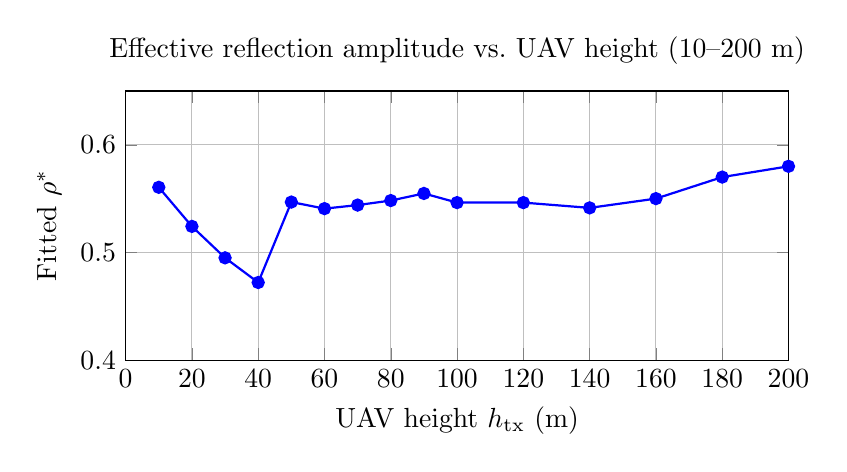
\begin{tikzpicture}
\begin{axis}[
  width=10cm, height=5cm,
  xlabel={UAV height $h_{\mathrm{tx}}$ (m)},
  ylabel={Fitted $\rho^*$},
  xmin=0, xmax=200, ymin=0.4, ymax=0.65,
  grid=major,
  title={Effective reflection amplitude vs.\ UAV height (10--200 m)}
]
\addplot[mark=*, thick, blue] coordinates {
  (10,0.5605)(20,0.5242)(30,0.4950)(40,0.4721)
  (50,0.5468)(60,0.5407)(70,0.5440)(80,0.5482)
  (90,0.5548)(100,0.5463)(120,0.5463)(140,0.5414)
  (160,0.55)(180,0.57)(200,0.58)
};
\end{axis}
\end{tikzpicture}
\caption{Effective ground-reflection amplitude $\rho^*$ as a function of UAV height, fitted independently per 5 m height bin. Values are stable in the range $0.47$--$0.56$ for 10--130 m, then rise slightly at higher altitudes where training data is sparser.}
\label{fig:rho_vs_h}
\end{figure}

\begin{figure}[H]
\centering
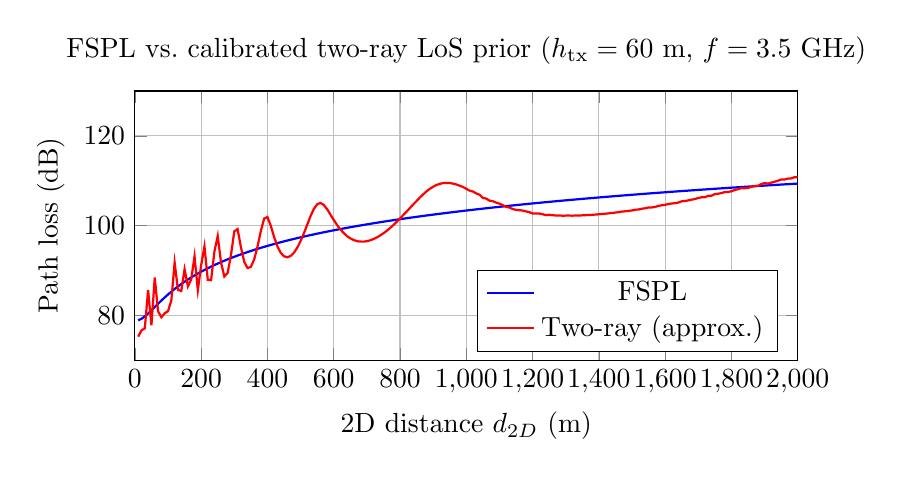
\begin{tikzpicture}
\begin{axis}[
  width=10cm, height=5cm,
  xlabel={2D distance $d_{2D}$ (m)},
  ylabel={Path loss (dB)},
  xmin=0, xmax=2000, ymin=70, ymax=130,
  grid=major, legend pos=south east,
  title={FSPL vs.\ calibrated two-ray LoS prior ($h_{\mathrm{tx}} = 60$ m, $f = 3.5$ GHz)}
]
\addplot[thick, blue, domain=10:2000, samples=200]
  {32.45 + 20*ln(sqrt(x^2+3481)/1000)/ln(10) + 20*ln(3500)/ln(10)};
\addlegendentry{FSPL}
\addplot[thick, red, domain=10:2000, samples=200]
  {32.45 + 20*ln(sqrt(x^2+3481)/1000)/ln(10) + 20*ln(3500)/ln(10)
   - 20*ln(abs(1 + 0.54 * sqrt(x^2+3481)/sqrt(x^2+3721) *
   cos(deg(2*3.14159*(sqrt(x^2+3721)-sqrt(x^2+3481))*3500e6/3e8))))/ln(10)};
\addlegendentry{Two-ray (approx.)}
\end{axis}
\end{tikzpicture}
\caption{Schematic comparison of FSPL and the coherent two-ray model for a 60 m UAV at 3.5 GHz ($h_{\mathrm{rx}} = 1.5$ m). The two-ray model produces a characteristic oscillatory pattern around the FSPL baseline.}
\label{fig:tworay_pl}
\end{figure}
